\chapter{Mechanizm zabezpieczaj�cy przed uszkodzeniem stanowiska}

W celu zabezpieczenia stanowiska w wypadku uszkodzenia czujnika (tj. $T1$ lub $T3$ przekroczy $250^{\circ}C$) zaimplementowano poni�ej przedstawiony (rys. \ref{safety_mechanism_code}) mechanizm zabezpieczaj�cy.

\begin{figure}[h!]
	\centering
	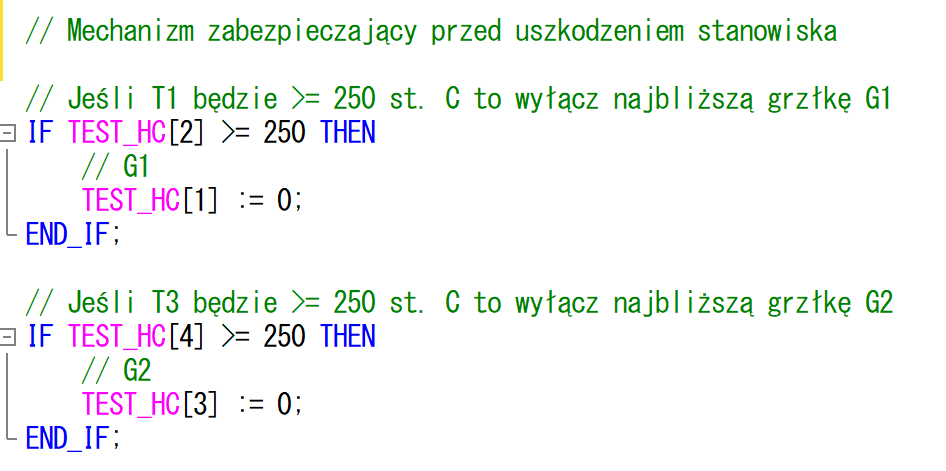
\includegraphics[width=\textwidth, center]{rysunki/SAFETY_MECHANISM_CODE.png}
	\caption{Kod zabezpieczaj�cy przed uszkodzeniem stanowiska grzej�co-ch�odz�cego}
	\label{safety_mechanism_code}
\end{figure}

\begin{figure}[h!b]
	\centering
	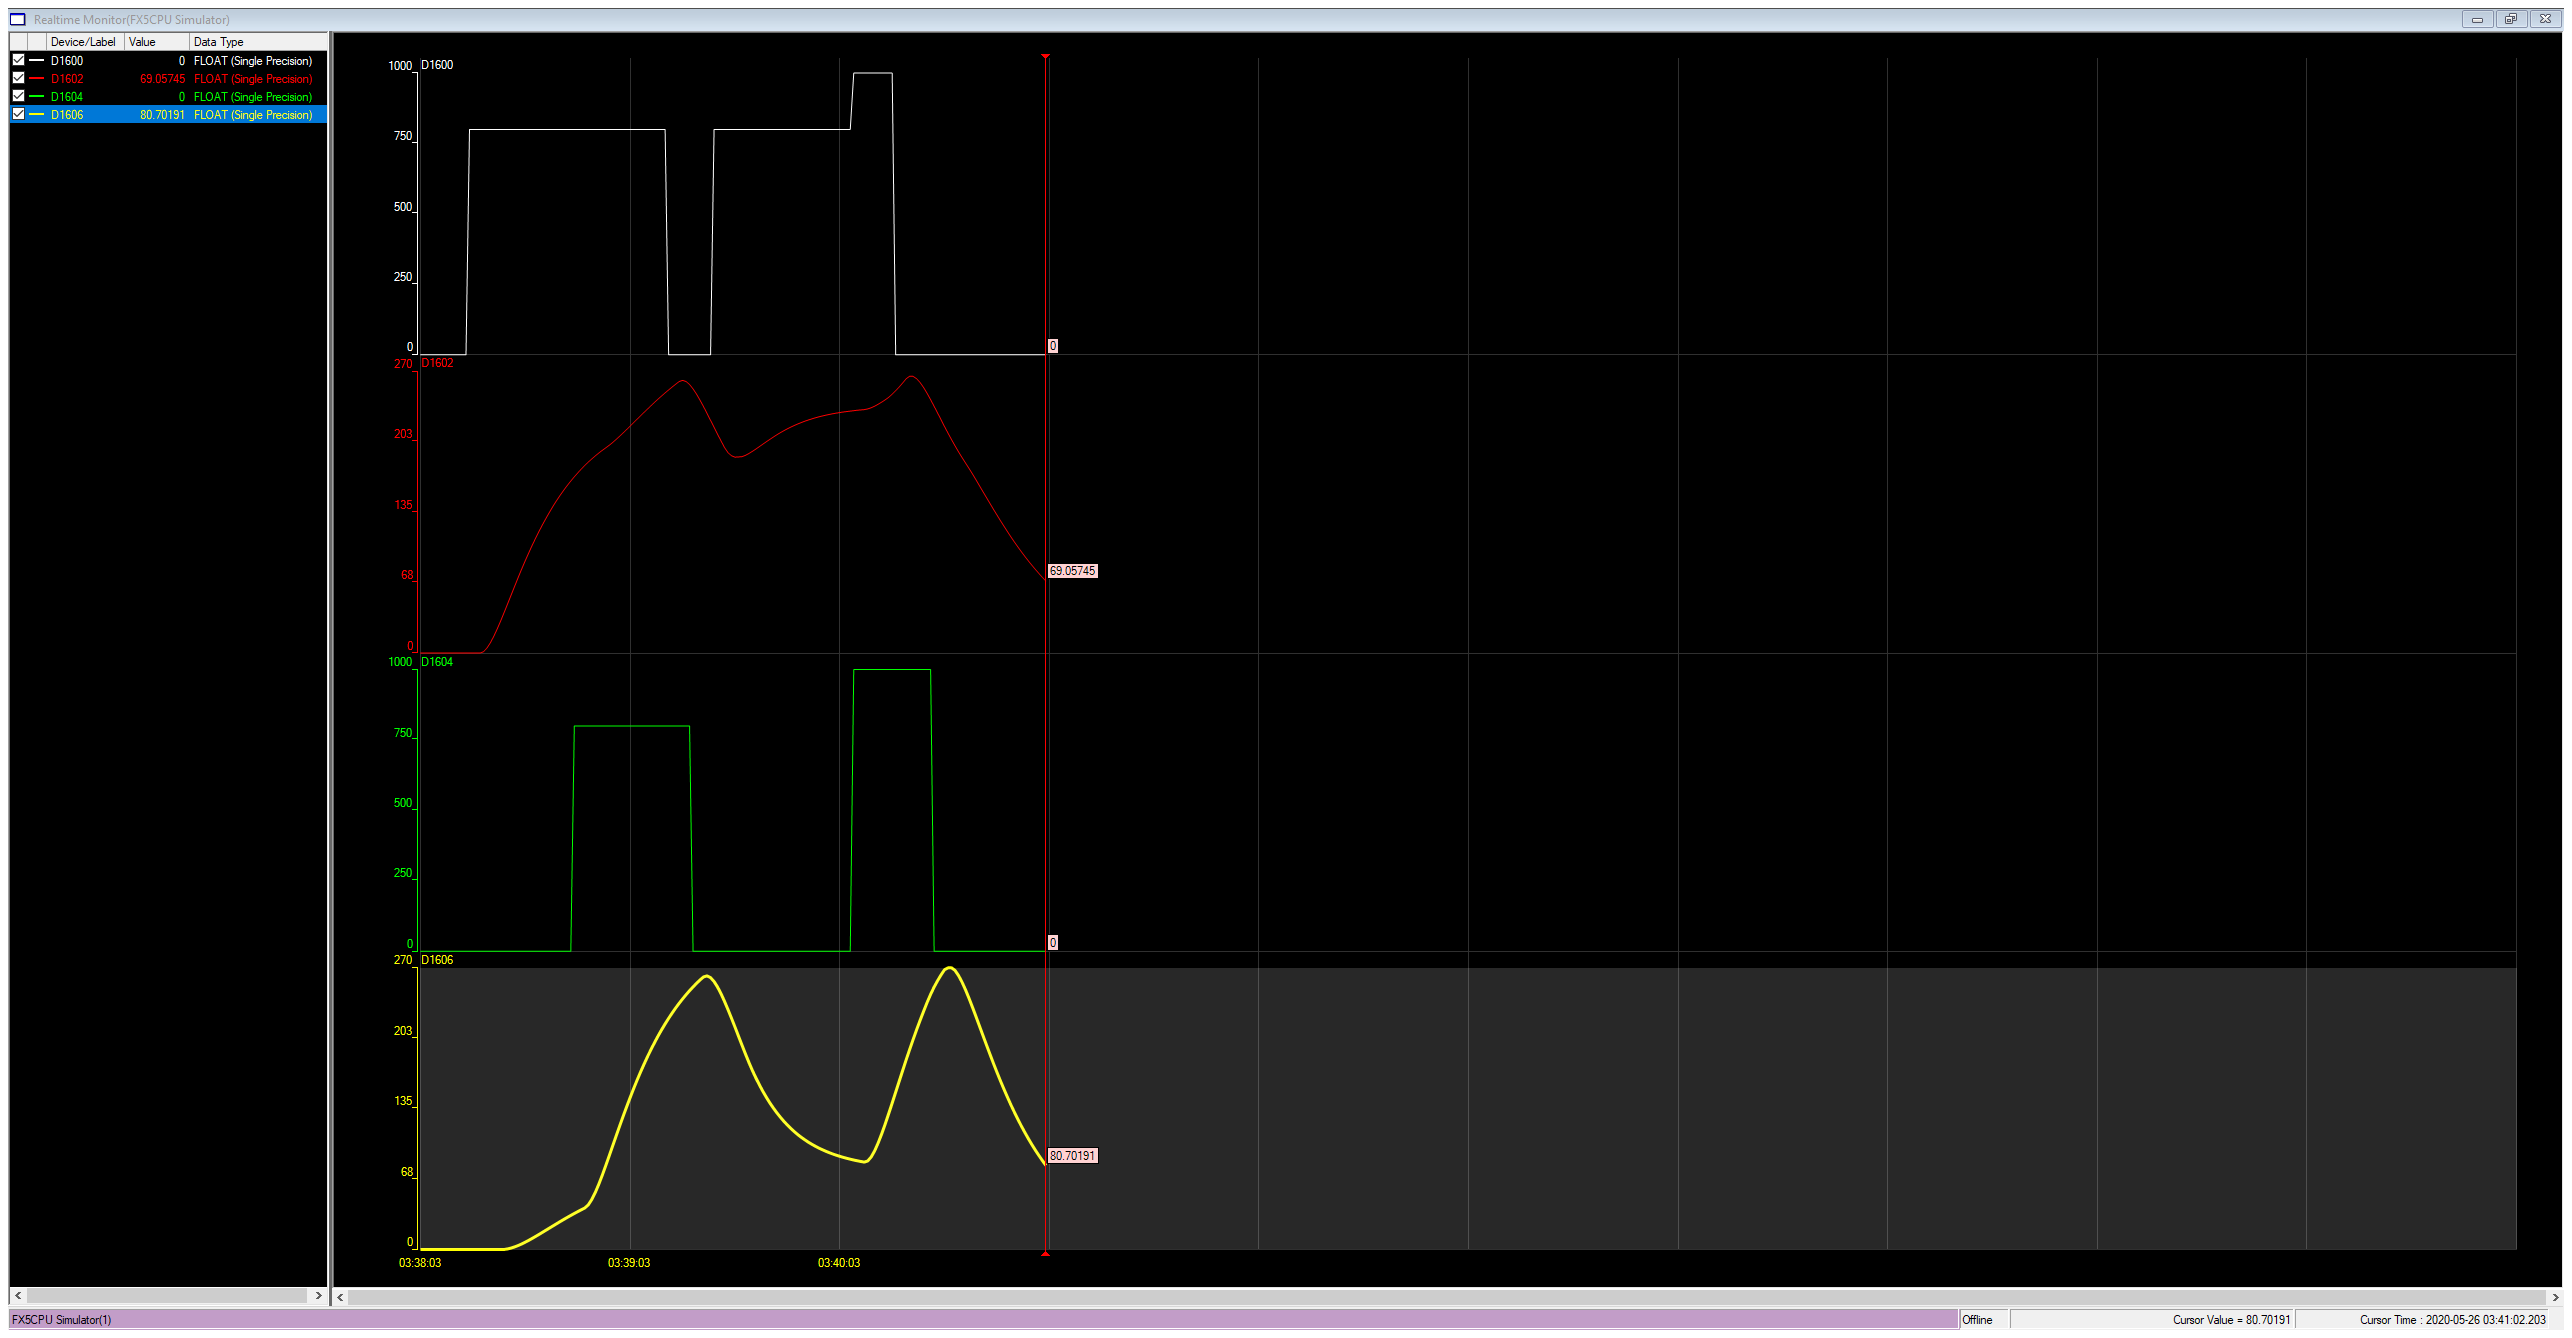
\includegraphics[clip, trim = 0 0 950 0, width=\textwidth, center]{rysunki/SAFETY_MECHANISM_FIGURE.png}
	\caption{Wykres prezentuj�cy dzia�anie mechanizmu zabezpieczaj�cego przed uszkodzeniem stanowiska grzej�co-ch�odz�cego}
	\label{safety_mechanism_figure}
\end{figure}

Jak widzimy na powy�szym rysunku (rys. \ref{safety_mechanism_figure}), gdy temperatura kt�rego� z wyj�� $T1$ lub $T3$ zaczyna przekracza� temperatur� $250^{\circ}C$ to odpowiednio wy��czane s� grza�ki $G1$ dla przekroczenia temperatury przez $T1$ i $G2$ dla przekroczenia temperatury przez $T3$. Dzi�ki temu grza�ka s�siaduj�ca z czujnikiem, kt�ry zmierzy� niebezpieczn� temperatur� zostanie wy��czona.